%%%%%%%%%%%%%%%%%%%%%%%%%%%%%%%%%%%%%%%%%%%%%%%%%%%%%%%%%%%%%%%%%%%%%%%%%%%%%%%%%%%%
% Do not alter this block (unless you're familiar with LaTeX
\documentclass{article}
\usepackage[margin=1in]{geometry} 
\usepackage{amsmath,amsthm,amssymb,amsfonts, fancyhdr, color, comment, graphicx, environ,minted}
\usepackage{xcolor}
\usepackage{graphicx}
\graphicspath{ {./images/} }
\usepackage{mdframed}
\usepackage{listings}
\usepackage[shortlabels]{enumitem}
\usepackage{indentfirst}
\usepackage{hyperref}
\hypersetup{
	colorlinks=true,
	linkcolor=blue,
	filecolor=magenta,      
	urlcolor=blue,
}


\pagestyle{fancy}


\newenvironment{problem}[2][Problem]
{ \begin{mdframed}[backgroundcolor=gray!20] \textbf{#1 #2} \\}
	{  \end{mdframed}}

% Define solution environment
\newenvironment{solution}{\textbf{Solution}}

%%%%%%%%%%%%%%%%%%%%%%%%%%%%%%%%%%%%%%%%%%%%%
%Fill in the appropriate information below
\lhead{NAME - STUDENT ID NUMBER}
\rhead{STAT6181} 
\chead{\textbf{ASSIGNMENT \#1}}
%%%%%%%%%%%%%%%%%%%%%%%%%%%%%%%%%%%%%%%%%%%%%

\renewcommand{\labelenumiii}{(\roman{enumiii})}
\begin{document}
	
	\textbf{Due Date: 23rd September 2021}
	
	Instructions:
	
	\begin{enumerate}
		\item Answer ALL questions in the spaces allocated.
		\item In this assignment, you are required to show all your working. 
		\item Your answers must be written in the spaces provided. You can adjust the spaces allocated for the answers if you need more space. You can type your answers if you wish. 
		\item \emph{\underline{The lecturer maintains the right to call students in individually and ask them questions on the assignments.}} 
		
		\emph{\underline{This may result in an adjustment of the final assignment grade.}}
		
		\item \emph{\underline{Upload  (i) Your R code (ii) Your Data and (3) A softcopy of your assignment on myelearning as a pdf. }} 
		
		\emph{\underline{In Dropbox 1. DO NOT SUBMIT AS A SINGLE ZIP FILE with all the documents.}}
	\end{enumerate}
	
	\vspace{2cm}
	
	\begin{enumerate}
		\item QUESTION 1  (OPTIMIZATION – function with two variables)
		\begin{enumerate}
			\item Do some reading on how you can find the maximum and minimum of a function f(x,y). You may come across terms like saddles point, partial derivatives etc. After you have read that, find the maximum, minimum and saddle points (if any) exists for the following function:
			
			$$
			f(x, y) = e^{-\frac{1}{3}x^2 + x - y^3}
			$$
			
			\hfill[10 marks]
			
			
			In order to find critical points (maxima, minima and saddle) of a multivariate function, we find partial derivatives with respect to each indivdual variable. From the above:
			\begin{equation*}
				f_{x}(x,y) = \left(-\frac{2}{3}x + 1\right)e^{-\frac{1}{3}x^2 + x - y^3}
			\end{equation*}
			\begin{equation*}
				f_{y}(x,y) = -3y^2 e ^{-\frac{1}{3}x^2 - y^3}
			\end{equation*}
			
			Both expressions are set to zero:
			\begin{equation*}
				\begin{split}
					f_{x}(x,y) &= 0\\
					\left(-\frac{2}{3}x + 1\right)e^{-\frac{1}{3}x^2 - y^3} &= 0
				\end{split} 
			\end{equation*}
			Since $e^{m}$ cannot be zero for all real values of m:
			\begin{equation*}
				\begin{split}
					e^{-\frac{1}{3}x^2 + x - y^3} &\neq 0\\
					\Rightarrow -\frac{2}{3}x + 1 &= 0\\
					\text{solving the above for }x\\
					x &= \frac{3}{2}
				\end{split} 
			\end{equation*}
			Doing the same for $f_{y}(x,y)$:
			\begin{equation*}
				\begin{split}
					f_{y}(x,y) &= 0\\
					-3y^2 e ^{-\frac{1}{3}x^2 + x - y^3} &= 0\\
				\end{split}
			\end{equation*}
			Following from the above, $e^m$ cannot be equal to zero for all real values of m:
			\begin{equation*}
				\begin{split}
					e ^{-\frac{1}{3}x^2 + x - y^3} &\neq 0\\
					\Rightarrow -3y^2 &= 0\\
					y &= 0
				\end{split}
			\end{equation*}
			
			From the above, $(\frac{3}{2}, 0)$ is a critical point in $f(x,y)$. To determine the nature of this critical point, we take the second derivative in both variables using chain rule:
			\begin{equation*}
				\begin{split}
					f_{x,x}(x,y) &= \left(-\frac{2}{3}x+1\right)^2\cdot e^{-\frac{1}{3}x^2 + x - y^3} + \left(-\frac{2}{3}\right) \left(e^{-\frac{1}{3}x^2 + x - y^3}\right)\\
					&= e^{-\frac{1}{3}x^2 + x - y^3}\left[\left(-\frac{2}{3}x+1\right)^2 -\frac{2}{3}\right]\\
					&= e^{-\frac{1}{3}x^2 + x - y^3}\left[-\frac{4}{9}x^2 -\frac{4}{3}x + \frac{1}{3}\right]
				\end{split}
			\end{equation*}
			Similarly:
			\begin{equation*}
				\begin{split}
					f_{y,y}(x,y) &= (-3y^2)^2\cdot e^{-\frac{1}{3}x^2 + x - y^3} - 6y\cdot e^{-\frac{1}{3}x^2 + x - y^3}\\
					&= (9y^4 - 6y)e^{-\frac{1}{3}x^2 + x - y^3}
				\end{split}
			\end{equation*}
			At critical point $(1.5, 0)$, $f_{x,x}(x,y) = -5.645$ and $f_{y,y}(x,y) = 0$. At this point, this may be inconclusive as $f_{y,y}(x,y) = 0$ at $(1.5, 0)$. Hence we use the second partials test the nature of the critical point, where:
			\begin{equation*}
				D = f_{xx} (x_{0}, y_0 )f_{yy} (x_{0}, y_{0}) - (f_{xy}(x_{0}, y_{0}))^2
			\end{equation*}
			We consider four case:
			\begin{enumerate}
				\item If $D>0$ and $f_{xx}(x_{0}, y_{0}) > 0$, then $f$ is concave up at this point and is therefore a local minimum
				\item If $D>0$ and $f_{xx}(x_{0}, y_{0}) < 0$, then $f$ is concave down at this point and is therefore a local maximum.
				\item If $D < 0$ then $f$ has a saddle point at $(x_0, y_0)$
				\item If $D=0$, then this test is inconclusive
			\end{enumerate}
			From the above, $f_{x}(x,y) = \left(-\frac{2}{3}x + 1\right)e^{-\frac{1}{3}x^2 + x - y^3}$, finding $f_{x,y}(x,y)$:
			\begin{equation*}
				\begin{split}
					f_{xy}(x,y) &= -3y^{2}\left(-\frac{2}{3}x + 1\right)e^{-\frac{1}{3}x^2 + x - y^3}
				\end{split}
			\end{equation*}
			Finding $f_{x,y}(x,y)$ at critical point $(1.5, 0)$:
			$f_{x,y}(1.5, 0) = 0$
			
			Hence $D = 0$
			\item Use R to plot a the function $f(x,y)$. Use the following range $ -2 < x < 2$  and $-2 < y < 2$.
			\begin{enumerate}
				\item Rcode   
				\begin{lstlisting}[language=R]
					# Specify range of x and y values
					xs <- seq(from = -2.0, to = 2.0, by = 0.5)
					ys <- seq(from = -2.0, to = 2.0, by = 0.5)
					
					#define the function
					fx <- function (x, y) {
						return (exp(-(1/3)*(x^2) + x - y^3))
					}
					# find matrix of values in both directions and apply function
					z <- outer(xs, ys, fx)
					
					# plot graph
					plot_ly(
					z = z, x=xs, y=ys, 
					type="contour", 
					colorscale='Bluered',
					width = 800, height = 500)
				\end{lstlisting}
				\hfill [2 marks]
				\item Plot
				
				
				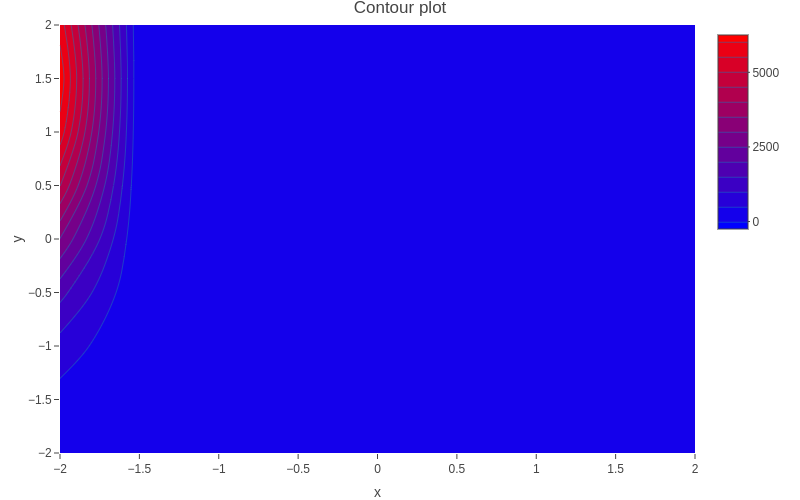
\includegraphics[width=8cm, height=5cm]{images/1b_ii_b.png}
				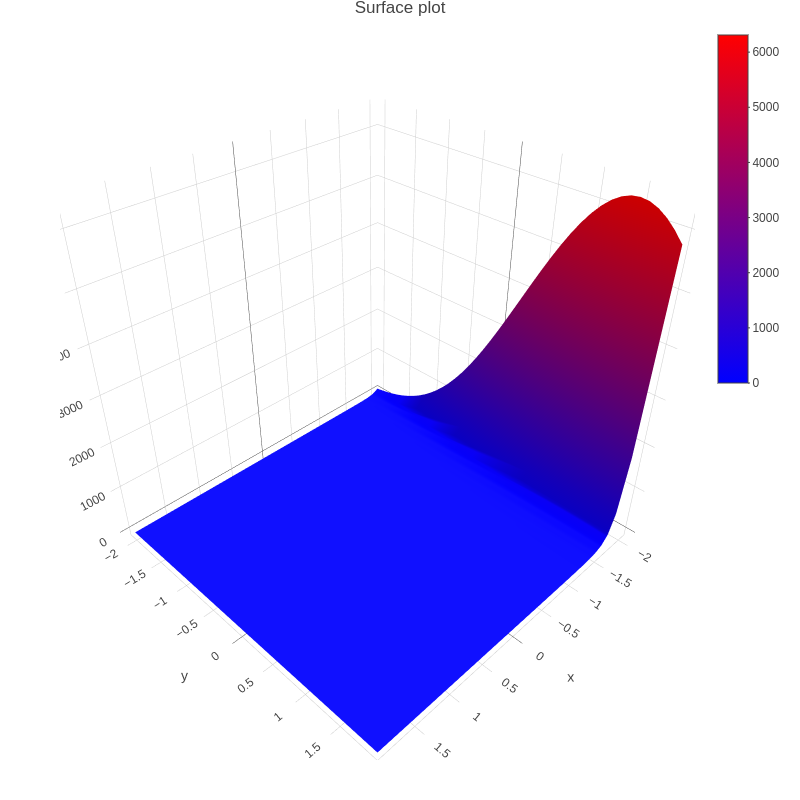
\includegraphics[width=7cm, height=7cm]{images/1b_ii_a.png}
				\hfill [2 marks]
			\end{enumerate}
			\item Use the optim function in R to confirm your results in (a).    
			\begin{enumerate}
				\item R code \& Output.
				
				\hfill [2 marks]
			\end{enumerate}
		\end{enumerate}
		\item Find the two parameter Weibull distribution in Wikipedia.
		\begin{enumerate}
			\item Write some R code to plot this distribution for the parameters $b = 5$ and $\eta = 1$.
			\begin{enumerate}
				\item R code 
				\begin{lstlisting}[language=R]
					library(ggplot2)
					library(plotly)
					
					weibull <- function(x, shape=1, scale=5) {
						(shape/scale)*(x/scale)^(shape-1)*exp(-(x/scale)^(shape))
					}
					
					x <- seq(0, 2, by=0.01)
					f_x <- weibull(x, shape=5, scale=1)
					
					data = data.frame(x, f_x)
					
					fig <- plot_ly(
					data, 
					x=x, 
					y=f_x, 
					name='2-param Weibull', 
					type='scatter', 
					mode='lines')
					
					fig <- fig %>% layout(
					title = '2-Parameter Weibull Distribution', 
					plot_bgcolor = "#e5ecf6")
					fig <- fig %>% layout(
					autosize = F, 
					width = 500, 
					height = 500, 
					margin = 0)
					
					fig
				\end{lstlisting}
				\hfill[1 mark]  
				\item Paste the plot here 
				
				
				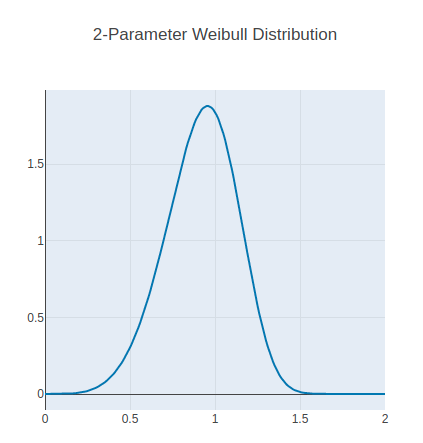
\includegraphics[width=7cm, height=7cm]{images/2a_ii.png}
				\hfill[1 mark]
				\item Use the newton’s method in the course handout and write suitable functions for $f, df$ and $df2$. Then generate 1,000 variates from a Weibull with $b = 5$ and $\eta = 1$ and check how well newton’s method is able to recover the estimates of the parameters.   You will follow the following steps to get this done:
				\begin{enumerate}
					\item code for generating the 1,000 variates from a Weibull with $b = 5$ and $\eta = 1$.   Use \texttt{set.seed(1123)} to ensure everyone has the same data.      
					\begin{lstlisting}[language=R]
						set.seed(1123)
						shape <- 5
						scale <- 1
						n <- 1000
						x <- rweibull(n, shape, scale)
					\end{lstlisting}
					\hfill [1 mark]
					
					\item Find the score vector (column of first derivatives).
					\newline
					
					The PDF of the Weibull is given by:
					$f(x|b, \eta) = \frac{\eta}/b \left(\frac{x}{b}\right) e^{-\left(\frac{x}{b}\right)^{\eta}} $
					
					The likelihood function is then found:
					$f(\widetilde{x}|b, \eta) = $
					
					Finding the natural logarithm of the above:
					
					$\mathcal{L} = n[\ln{\eta} - \eta\ln{b}] + (\eta - 1)\sum_{i=1}^{n}\ln{X_{i}} - \sum_{i=1}^{n}(X_{i}/b)^{\eta}$
					\newline
					
					To find the vector of score functions, the partial derivatives of the above need be found:
					
					\begin{equation*}
						\begin{split}
							\frac{\delta^{2}\mathcal{L}}{\delta \eta^{2}} &= \frac{b}{\eta^2}\left[n+(b + 1)\sum_{i=1}^{n}\frac{X_{i}}{\eta}^{b}\right]\\
							\frac{\delta^{2}\mathcal{L}}{\delta b^{2}} &= \frac{n}{b^{2}} - \sum_{i=1}^{n} \frac{X_{i}}{\eta}^{b}\left[\ln{\frac{X_{i}}{\eta}}\right]^2\\
							\frac{\delta^{2}\mathcal{L}}{\delta b \delta\eta} =  \frac{\delta^{2}\mathcal{L}}{\delta\eta\delta b} &= \frac{1}{\eta}\left[n - \sum_{i=1}^{n}\left(\frac{X_{i}}{\eta}\right)^{b}\ln{\frac{X_{i}}{\eta}}^2\right]
						\end{split}
					\end{equation*}
					
					
					\hfill [4 marks]
					
					\item Write an R function for the first derivatives $(df)$ which you will use in the Newton Raphson method.   \begin{lstlisting}[language=R]
						df <- function(t) {
							eta <- t[1]
							b <- t[2]
							
							score = rep(0,2)
							score[1] = -(n*b)/eta + (b/eta)*sum((x/eta)^b )
							score[2] = n/b-n*log(eta)+sum(log(x))-sum((x/eta)^(b)*log(x/eta))
							
							return(score)
						}
					\end{lstlisting}
					\hfill[ 4 marks]
					
					\item Find the hessian matrix (matrix of second derivatives which we call $df2$).       
					To find the Hessian matrix, the second partial derivatives with respect to both $\eta$ and $b$ need be found:
					\begin{equation*}
						\begin{split}
							\frac{\delta^{2}\mathcal{L}}{\delta b^{2}} &= \frac{\eta}{b^2}\left[n-(\eta - 1)\sum_{i=1}^{n}\frac{X_{i}}{b}^{\eta}\right]\\
							\frac{\delta^{2}\mathcal{L}}{\delta \eta^{2}} &= \frac{n}{\eta^{2}} - \sum_{i=1}^{n} \frac{X_{i}}{b}^{\eta}\left[\ln{\frac{X_{i}}{b}}\right]^2\\
							\frac{\delta^{2}\mathcal{L}}{\delta b \delta\eta} =  \frac{\delta^{2}\mathcal{L}}{\delta\eta\delta b} &= -\frac{1}{b}\left[n - \sum_{i=1}^{n}\frac{X_{i}}{b}^{\eta} - \eta\sum_{i=1}^{n}\left(\frac{X_{i}}{b}\right)^{\eta}\ln{\frac{X_{i}}{b}}\right]
						\end{split}
					\end{equation*}
					\hfill[ 4 marks]
					\item Write an R function for the hessian matrix $(df2)$ which you will use in the newton Raphson method.
					\begin{lstlisting}[language=R]
						df2 <- function(t) {
							eta <- t[1]
							b <- t[2]
							
							h <- matrix(0,2,2)    
							h[1,1] <- n*b/eta^2 + (b*(b+1))/(eta^2) * sum((x/eta)^b)
							h[2,2] <- n/b^2 - sum((x/eta)^b * (log(x/eta))^2)
							h[1,2] <- n/eta - (1/eta)*sum((x/eta)^(b) *log(x/eta)^(2))
							h[2,1] <- h[1,2]
							
							return(h)
						}
					\end{lstlisting}
					\hfill[ 4 marks]
					\item Apply the Newton Raphson Method in R and give the output. Comment on your results.   
					\hfill[ 4 marks]
				\end{enumerate}
			\end{enumerate}
		\end{enumerate}
	\end{enumerate}
	
	% \section*{\centering }
	% \begin{problem}{a}
	%     (a)	
	
	% \end{problem}
	% \vspace{1cm}
	% \begin{solution}
	
	% \end{solution}
	
	
\end{document}